\documentclass[alternative-exam.tex]{subfiles}
\begin{document}

\chapter{Wisselkoers}
\begin{figure}[H]
\label{rushour}
\caption{Opgave}
\begin{center}
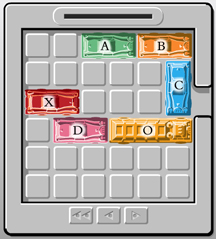
\includegraphics[scale=1.25]{figure-rushour.jpg}
\end{center}
\end{figure}

\section{Vraag}
Rush hour is een schuifpuzzel die een verkeersopstopping voorstelt. Het doel is om de rode auto (X) uit het verkeer te krijgen in zo weinig mogelijk zetten. De andere auto's staan in de weg en elke auto kan enkel vooruit en achteruit bewegen. Auto's mogen meerdere vakjes per keer verschuiven maar er mag maar één auto per zet verplaatst worden.\\\\
Beschouw elke stand van het bord als een toestand van de zoekruimte. Beschouw bovendien elke mogelijke zet als een boog in het netwerk. De begintoestand is gegeven in figuur \ref{rushour}. De eindtoestand is een toestand waarin de rode auto zich buiten het bord bevindt. De kostfunctie kan informeel beschreven worden als het aantal benodigde zetten. Als heuristiek kiezen we het kleinste aantal auto's dat onbeweeglijk in de weg staat van de rode auto\footnote{BvB. De heuristische waarde van de root is $3$ want $C$ staat in de weg van de rode auto en om $C$ te verplaatsen moeten er minstens $2$ auto's verplaatst worden, namelijk $A$ en $B$ of $O$ en $D$.  }.

\section{Modeloplossing}
De volgende tabel stelt de begintoestand voor. Deze toestand is de wortel die initieel in de rij staat.
\begin{center}
$root = $
\begin{tabular}{| c | c | c | c | c | c |}
\hline
   &   & A & A & B & B \\ \hline
   &   &   &   &   & C \\ \hline
 X & X &   &   &   & C \\ \hline
   & D & D & O & O & O \\ \hline
   &   &   &   &   &   \\ \hline
   &   &   &   &   &   \\
\hline
\end{tabular}
\end{center}

\subsection{Iteratie 1}
We starten nu de while-lus van het algoritme. We expanderen alle mogelijke toestanden die in 1 zet bereikbaar zijn vanaf de begintoestand. Die toestanden zetten we allemaal op de queue. We expanderen de nodes in volgorde van het alfabet en altijd de mogelijkheid waarin het autootje de grootste afstand aflegt eerst.

\begin{center}
$T_{11} = $
\scalebox{0.5}{
\begin{tabular}{| p{0.3cm} | p{0.3cm} | p{0.3cm} | p{0.3cm} | p{0.3cm} | p{0.3cm} |}
\hline
 A & A &   &   & B & B \\ \hline
   &   &   &   &   & C \\ \hline
 X & X &   &   &   & C \\ \hline
   & D & D & O & O & O \\ \hline
   &   &   &   &   &   \\ \hline
   &   &   &   &   &   \\
\hline
\end{tabular}}
$T_{12} = $
\scalebox{0.5}{
\begin{tabular}{| p{0.3cm} | p{0.3cm} | p{0.3cm} | p{0.3cm} | p{0.3cm} | p{0.3cm} |}
\hline
   & A & A &   & B & B \\ \hline
   &   &   &   &   & C \\ \hline
 X & X &   &   &   & C \\ \hline
   & D & D & O & O & O \\ \hline
   &   &   &   &   &   \\ \hline
   &   &   &   &   &   \\
\hline
\end{tabular}}
$T_{13} = $
\scalebox{0.5}{
\begin{tabular}{| p{0.3cm} | p{0.3cm} | p{0.3cm} | p{0.3cm} | p{0.3cm} | p{0.3cm} |}
\hline
   &   & A & A & B & B \\ \hline
   &   &   &   &   & C \\ \hline
 X & X &   &   &   & C \\ \hline
 D & D &   & O & O & O \\ \hline
   &   &   &   &   &   \\ \hline
   &   &   &   &   &   \\
\hline
\end{tabular}}
\end{center}

\begin{center}
$T_{14} = $
\scalebox{0.5}{
\begin{tabular}{| p{0.3cm} | p{0.3cm} | p{0.3cm} | p{0.3cm} | p{0.3cm} | p{0.3cm} |}
\hline
   &   & A & A & B & B \\ \hline
   &   &   &   &   & C \\ \hline
   &   &   & X & X & C \\ \hline
   & D & D & O & O & O \\ \hline
   &   &   &   &   &   \\ \hline
   &   &   &   &   &   \\
\hline
\end{tabular}}
$T_{15} = $
\scalebox{0.5}{
\begin{tabular}{| p{0.3cm} | p{0.3cm} | p{0.3cm} | p{0.3cm} | p{0.3cm} | p{0.3cm} |}
\hline
   &   & A & A & B & B \\ \hline
   &   &   &   &   & C \\ \hline
   &   & X & X &   & C \\ \hline
   & D & D & O & O & O \\ \hline
   &   &   &   &   &   \\ \hline
   &   &   &   &   &   \\
\hline
\end{tabular}}
$T_{16} = $
\scalebox{0.5}{
\begin{tabular}{| p{0.3cm} | p{0.3cm} | p{0.3cm} | p{0.3cm} | p{0.3cm} | p{0.3cm} |}
\hline
   &   & A & A & B & B \\ \hline
   &   &   &   &   & C \\ \hline
   & X & X &   &   & C \\ \hline
   & D & D & O & O & O \\ \hline
   &   &   &   &   &   \\ \hline
   &   &   &   &   &   \\
\hline
\end{tabular}}
\end{center}
Geen enkele van deze toestanden is beschrijft een cyclus in het netwerk. De rij moet nu nog gesorteerd worden op de $f$ functie. Aangezien elke zet dezelfde kost heeft, namelijk $1$, is dat sorteren equivalent aan het sorteren op de heuristische waarde van elke toestand.
\[
\begin{array}{c c}
f(T_{11}) &= 1+ 2 = 3\\
f(T_{12}) &= 1+ 2 = 3\\
f(T_{13}) &= 1+ 2 = 3\\
f(T_{14}) &= 1+ 3 = 4\\
f(T_{15}) &= 1+ 3 = 4\\
f(T_{16}) &= 1+ 3 = 4\\
\end{array}
\]
De rij ziet er na deze stap als volgt uit.
\[
Q_1 = \{X_{11},T_{12},T_{13},T_{14},T_{15},T_{16}\}
\]
\subsection{Iteratie 2}
Om de volgende iteratie te beginnen, halen we het element met de kleinste $f$-waarde uit de rij (het eerste element). In dit geval is dit $T_{11}$. We expanderen deze toestand en verkrijgen de volgende mogelijke toestanden.
\begin{center}
$T_{21} = $
\scalebox{0.5}{
\begin{tabular}{| p{0.3cm} | p{0.3cm} | p{0.3cm} | p{0.3cm} | p{0.3cm} | p{0.3cm} |}
\hline
   &   & A & A & B & B \\ \hline
   &   &   &   &   & C \\ \hline
 X & X &   &   &   & C \\ \hline
   & D & D & O & O & O \\ \hline
   &   &   &   &   &   \\ \hline
   &   &   &   &   &   \\
\hline
\end{tabular}}
$T_{22} = $
\scalebox{0.5}{
\begin{tabular}{| p{0.3cm} | p{0.3cm} | p{0.3cm} | p{0.3cm} | p{0.3cm} | p{0.3cm} |}
\hline
   & A & A &   & B & B \\ \hline
   &   &   &   &   & C \\ \hline
 X & X &   &   &   & C \\ \hline
   & D & D & O & O & O \\ \hline
   &   &   &   &   &   \\ \hline
   &   &   &   &   &   \\
\hline
\end{tabular}}
$T_{23} = $
\scalebox{0.5}{
\begin{tabular}{| p{0.3cm} | p{0.3cm} | p{0.3cm} | p{0.3cm} | p{0.3cm} | p{0.3cm} |}
\hline
 A & A & B & B &   &   \\ \hline
   &   &   &   &   & C \\ \hline
 X & X &   &   &   & C \\ \hline
   & D & D & O & O & O \\ \hline
   &   &   &   &   &   \\ \hline
   &   &   &   &   &   \\
\hline
\end{tabular}}
\end{center}
\begin{center}
$T_{24} = $
\scalebox{0.5}{
\begin{tabular}{| p{0.3cm} | p{0.3cm} | p{0.3cm} | p{0.3cm} | p{0.3cm} | p{0.3cm} |}
\hline
 A & A &   & B & B &   \\ \hline
   &   &   &   &   & C \\ \hline
 X & X &   &   &   & C \\ \hline
   & D & D & O & O & O \\ \hline
   &   &   &   &   &   \\ \hline
   &   &   &   &   &   \\
\hline
\end{tabular}}
$T_{25} = $
\scalebox{0.5}{
\begin{tabular}{| p{0.3cm} | p{0.3cm} | p{0.3cm} | p{0.3cm} | p{0.3cm} | p{0.3cm} |}
\hline
 A & A &   &   & B & B \\ \hline
   &   &   &   &   & C \\ \hline
 X & X &   &   &   & C \\ \hline
 D & D &   & O & O & O \\ \hline
   &   &   &   &   &   \\ \hline
   &   &   &   &   &   \\
\hline
\end{tabular}}
$T_{26} = $
\scalebox{0.5}{
\begin{tabular}{| p{0.3cm} | p{0.3cm} | p{0.3cm} | p{0.3cm} | p{0.3cm} | p{0.3cm} |}
\hline
 A & A &   &   & B & B \\ \hline
   &   &   &   &   & C \\ \hline
   &   &   & X & X & C \\ \hline
   & D & D & O & O & O \\ \hline
   &   &   &   &   &   \\ \hline
   &   &   &   &   &   \\
\hline
\end{tabular}}
\end{center}
\begin{center}3
$T_{27} = $
\scalebox{0.5}{
\begin{tabular}{| p{0.3cm} | p{0.3cm} | p{0.3cm} | p{0.3cm} | p{0.3cm} | p{0.3cm} |}
\hline
 A & A &   &   & B & B \\ \hline
   &   &   &   &   & C \\ \hline
   &   & X & X &   & C \\ \hline
   & D & D & O & O & O \\ \hline
   &   &   &   &   &   \\ \hline
   &   &   &   &   &   \\
\hline
\end{tabular}}
$T_{28} = $
\scalebox{0.5}{
\begin{tabular}{| p{0.3cm} | p{0.3cm} | p{0.3cm} | p{0.3cm} | p{0.3cm} | p{0.3cm} |}
\hline
 A & A &   &   & B & B \\ \hline
   &   &   &   &   & C \\ \hline
   & X & X &   &   & C \\ \hline
   & D & D & O & O & O \\ \hline
   &   &   &   &   &   \\ \hline
   &   &   &   &   &   \\
\hline
\end{tabular}}
\end{center}
Wanneer we nu deze nieuwe toestanden nakijken om te zien of er geen cycli zijn gevormd, zien we dat $T_{21} = root$. Dit betekent dat we $T_{21}$ al mogen verwijderen. We zetten de andere toestanden bij in de rij en sorteren deze weer.
\[
\begin{array}{c c}
f(T_{22}) &= 2+ 2 = 4\\
f(T_{23}) &= 2+ 1 = 3\\
f(T_{24}) &= 2+ 1 = 3\\
f(T_{25}) &= 2+ 2 = 4\\
f(T_{26}) &= 2+ 2 = 4\\
f(T_{27}) &= 2+ 2 = 4\\
f(T_{28}) &= 2+ 2 = 4\\
\end{array}
\]
We verkrijgen dan de volgende rij.
\[
Q_2 = \{T_{23}, T_{24}, T_{12},T_{13},T_{22}, T_{25}, T_{26}, T_{27}, T_{28}, T_{14},T_{15},T_{16}\}
\]

\section{Iteratie 3}
Het volgende element dat we moeten expanderen is $T_{23}$. Wanneer we dit doen zien we dat we al vrij dicht bij de gewenste uitkomst komen. De volgende toestanden zijn de toestanden die bereikbaar zijn vanuit $T_{23}$.
\begin{center}
$T_{31} = $
\scalebox{0.5}{
\begin{tabular}{| p{0.3cm} | p{0.3cm} | p{0.3cm} | p{0.3cm} | p{0.3cm} | p{0.3cm} |}
\hline
 A & A &   &   & B & B \\ \hline
   &   &   &   &   & C \\ \hline
 X & X &   &   &   & C \\ \hline
   & D & D & O & O & O \\ \hline
   &   &   &   &   &   \\ \hline
   &   &   &   &   &   \\
\hline
\end{tabular}}
$T_{32} = $
\scalebox{0.5}{
\begin{tabular}{| p{0.3cm} | p{0.3cm} | p{0.3cm} | p{0.3cm} | p{0.3cm} | p{0.3cm} |}
\hline
 A & A &   & B & B &   \\ \hline
   &   &   &   &   & C \\ \hline
 X & X &   &   &   & C \\ \hline
   & D & D & O & O & O \\ \hline
   &   &   &   &   &   \\ \hline
   &   &   &   &   &   \\
\hline
\end{tabular}}
$T_{33} = $
\scalebox{0.5}{
\begin{tabular}{| p{0.3cm} | p{0.3cm} | p{0.3cm} | p{0.3cm} | p{0.3cm} | p{0.3cm} |}
\hline
 A & A & B & B &   & C \\ \hline
   &   &   &   &   & C \\ \hline
 X & X &   &   &   &   \\ \hline
   & D & D & O & O & O \\ \hline
   &   &   &   &   &   \\ \hline
   &   &   &   &   &   \\
\hline
\end{tabular}}
\end{center}
\begin{center}
$T_{34} = $
\scalebox{0.5}{
\begin{tabular}{| p{0.3cm} | p{0.3cm} | p{0.3cm} | p{0.3cm} | p{0.3cm} | p{0.3cm} |}
\hline
 A & A & B & B &   &   \\ \hline
   &   &   &   &   & C \\ \hline
 X & X &   &   &   & C \\ \hline
 D & D &   & O & O & O \\ \hline
   &   &   &   &   &   \\ \hline
   &   &   &   &   &   \\
\hline
\end{tabular}}
$T_{35} = $
\scalebox{0.5}{
\begin{tabular}{| p{0.3cm} | p{0.3cm} | p{0.3cm} | p{0.3cm} | p{0.3cm} | p{0.3cm} |}
\hline
 A & A & B & B &   &   \\ \hline
   &   &   &   &   & C \\ \hline
   &   &   & X & X & C \\ \hline
   & D & D & O & O & O \\ \hline
   &   &   &   &   &   \\ \hline
   &   &   &   &   &   \\
\hline
\end{tabular}}
$T_{36} = $
\scalebox{0.5}{
\begin{tabular}{| p{0.3cm} | p{0.3cm} | p{0.3cm} | p{0.3cm} | p{0.3cm} | p{0.3cm} |}
\hline
 A & A & B & B &   &   \\ \hline
   &   &   &   &   & C \\ \hline
   &   & X & X &   & C \\ \hline
   & D & D & O & O & O \\ \hline
   &   &   &   &   &   \\ \hline
   &   &   &   &   &   \\
\hline
\end{tabular}}
\end{center}
\begin{center}
$T_{37} = $
\scalebox{0.5}{
\begin{tabular}{| p{0.3cm} | p{0.3cm} | p{0.3cm} | p{0.3cm} | p{0.3cm} | p{0.3cm} |}
\hline
 A & A & B & B &   &   \\ \hline
   &   &   &   &   & C \\ \hline
   & X & X &   &   & C \\ \hline
   & D & D & O & O & O \\ \hline
   &   &   &   &   &   \\ \hline
   &   &   &   &   &   \\
\hline
\end{tabular}}
\end{center}
We zien dat $T_{34}$ een cyclus vormt met $T_{12}$. Deze toestand mag dus al verwijderd worden.
\[
\begin{array}{c c}
f(T_{31}) &= 3+ 2 = 5\\
f(T_{32}) &= 3+ 1 = 4\\
f(T_{33}) &= 3+ 0 = 3\\
f(T_{35}) &= 3+ 1 = 4\\
f(T_{36}) &= 3+ 1 = 4\\
f(T_{37}) &= 3+ 1 = 4\\
\end{array}
\]
Als we deze toestanden toevoegen aan de rij en deze opnieuw sorteren, krijgen we de volgende rij.
\[
Q_3 = \{T_{33}, T_{23}, T_{24}, T_{12}, T_{13}, T_{32}, T_{35}, T_{36}, T_{37}, T_{22}, T_{25}, T_{26}, T_{27}, T_{28}, T_{14},T_{15},T_{16}, T_{31}\}
\]

\section{Iteratie 4}



\end{document}